\documentclass[main]{subfiles}
\begin{document}

%@@@@@@@@@@@@@@@@@@@@@@@@@@@@@@
% Main Topics: Hopfield Networks 20.12.2018
% Lecturer: Matthew Cook
% author: Vanessa Leite - base document from benelot/eth-intro-to-neuroinformatics-summary

\section{Hopfield Networks}

\begin{itemize}[noitemsep,nolistsep]
	\item Every node is connected to every other node but not to itself.
	\item Connection weights are symmetric.
	\item $\sum x_i w_i < 0$ is disabled, $\sum x_i w_i \geq 0$ is enabled.
	\item Entire Network is in some state at any time. Set of active units of the entire network is important.
	\item Some states are stable and some are not. While in an unstable state, updating the network leads to a state change.
	\item Stable state is a local minimum. This does however not have to happen.
	\item Bias is an unit that is always on.
	\item Weight of a connection is correlated to frequency of firing together (Hebbian learning).
\end{itemize}

It seems that our memory works with Pattern Completion, also known as Content Addressable Memory or Associative Memory.
This memory has no input-output relation: given any piece of it, we can recover the rest.

\subsection{Hopfield and Memory}
\begin{itemize}[noitemsep,nolistsep]
	\item A hopfield network is an associative type of memory. Information is stored in the stable states as local minima.
	\item It is important that information is distinct.
	\item Associative memory has room for error but is still recognizable. Convergence to nearby stable states.
	\item Only helpful if reliable input.
	\item If some units are retrievable and all others are set randomly, the correct units will eventually set wrong units right.
\end{itemize}

\begin{figure}[H]
	\centering
	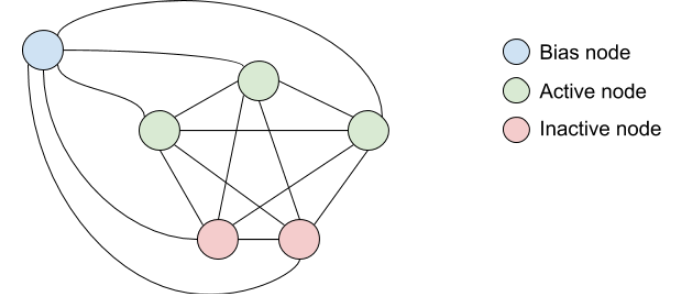
\includegraphics[width=0.3\textwidth]{hopfield-network-basic.png}
\end{figure}

\subsection{Updates and State Dynamics}

Maximize the sum of active weights (weights between active units) is the dynamic of Hopfield network (updating the output of one unit at time). This results in a stable state. We update everything but the bias node.

Mathematically, we can consider active units as a "+1" and inactive units as "-1". Remember, here, inactive neurons don't send inhibitory signal.
With this new representation, the hopfield network dynamic is equivalent to a graph min-cut, i.e., we want to minimize the sum of weights that link active and inactive units.

The above method is asynchronous.
Let's consider a synchronous case (updating all units at the same time): active units for time $t+1$ are computed on active units at time $t$.

\begin{figure}[H]
	\centering
	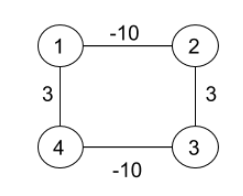
\includegraphics[width=0.3\textwidth]{synchronous-hopfield.png}
	\caption{Starting with 1 and 2 actives, in the next step 3 and 4 will be active. This network is not stable.}
\end{figure}

Trick for analysis: make a larger asynchronous network based on the network we want to analyse. Duplicate the units in two columns and only use non-zero weights between them.

\begin{figure}[H]
	\centering
	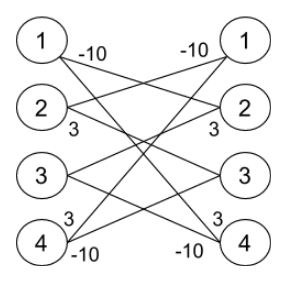
\includegraphics[width=0.3\textwidth]{hopfield-asynchronous-trick.png}
	\caption{Starting with 1 and 2 actives, we will end up with 3 and 4 active in the second column. First column represents $t=0$, second $t=1$. With synchronous updates, a Hopfield network converges to a cycle of length 2 or 1.}
\end{figure}

\begin{itemize}[noitemsep,nolistsep]
	\item Nodes can be updated synchronously or asynchronously.
	\item State: Set of units that are active.
	\item Dynamics: Units update their activity level.
	\item When a node is updated, weights are considered from all other active nodes, like with a perceptron.
	\item Asynchronous updates (greedy algorithm) converge to a stable state (sequential), but the converged state can depend on update order.
	\item Asynchronous is either in max-clique state if activity is in $\{0,1\}$ or min-cut if activities are in $\{-1,1\}$.
	\item Synchronous, parallel updates either also go to a stable state, just like asynchronous, or can get stuck in a pair of patterns (flipping or cyclic).
\end{itemize}

\subsubsection{Perceptive Visual Field}

A neuron is "tuned" to a moving bar at a certani angle in its perceptive field. It also responds to a certain velocity, position (x,y), bar width, etc.

Neurons response is called firing rates. Although neurons are tuned, they aren't super picky about the exact values. And, experimentally, neurons do not code a single atributte but a combination of them.

\paragraph{Population code}

Information is encoded by a group (population) of neurons. A group includes all neurons in that area. The values are encoded by pattern of activity.

\begin{itemize}[noitemsep,nolistsep]
	\item Neurons can represent information through population codes.
	\item Neurons are tuned to preferred stimuli.
	\item Information is represented by the pattern of activity in a neural population.
	\item Each neuron has a preferred input, for example orientation, that it responds to. The neuron is tuned to that value.
	\item Not every neuron shows clear tuning curves.
	\item Neurons usually do not only respond to their preferred stimulus, but also with decaying strength to close ones.
\end{itemize}

\begin{figure}[H]
	\centering
	\begin{subfigure}[b]{0.3\textwidth}
		\centering
		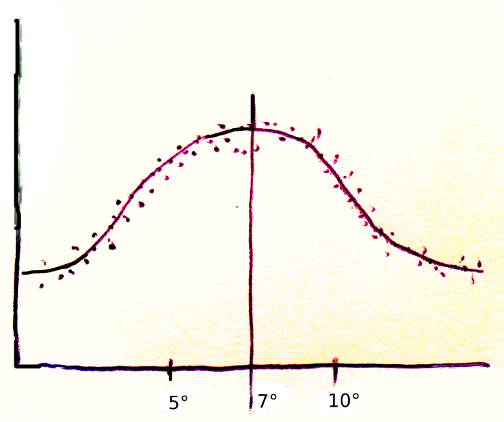
\includegraphics[width=\textwidth]{one-cell-tuning-curve.png}
		\caption{Tuning curve of one cell}
	\end{subfigure}%
	~
	\begin{subfigure}[b]{0.3\textwidth}
		\centering
		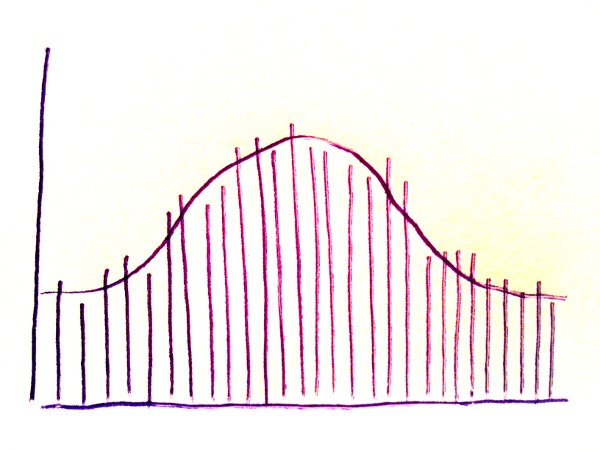
\includegraphics[width=\textwidth]{cell-order.png}
		\caption{Cells ordered by response to $20^\circ$}
	\end{subfigure}
	~ 
	\begin{subfigure}[b]{0.3\textwidth}
		\centering
		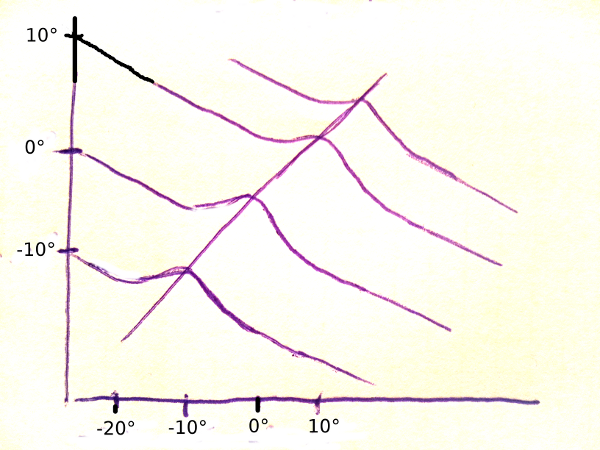
\includegraphics[width=\textwidth]{3D-visualisation.png}
		\caption{3D visualization of cell's response to different degrees}
	\end{subfigure}
\end{figure}

\begin{figure}[H]
	\centering
	\begin{subfigure}[b]{0.5\textwidth}
		\centering
		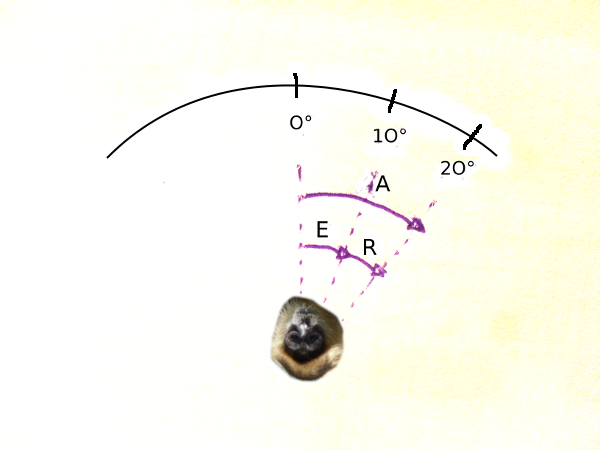
\includegraphics[width=\textwidth]{ape-picture.png}
		\caption{Monkey holding gaze fixed on point $10^\circ$ and light falling in from $20^\circ$}
	\end{subfigure}%
	~
	\begin{subfigure}[b]{0.5\textwidth}
		\centering
		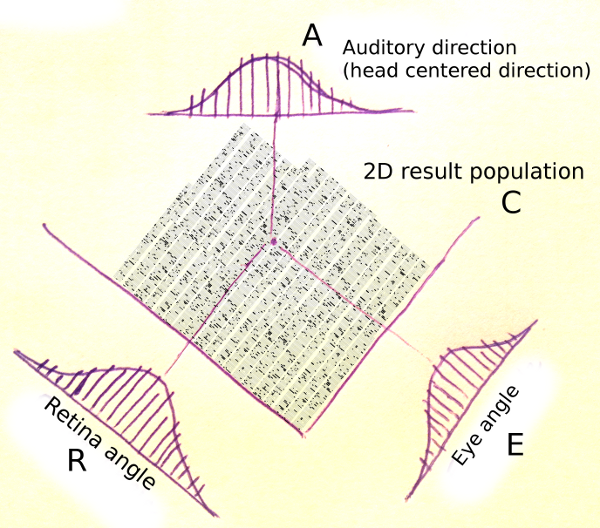
\includegraphics[width=\textwidth]{Retina-Eye-Auditory.png}
		\caption{Visualization of Retina angle ordering cell set R, Eye angle ordering set E,2D result population C and auditory direction set A.}
		\label{fig:population}
	\end{subfigure}
\end{figure}

\begin{figure}[H]
	\centering
	\begin{subfigure}[b]{0.3\textwidth}
		\centering
		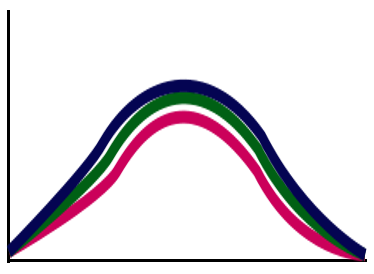
\includegraphics[width=\textwidth]{Cell-A.png}
		\caption{Cell A $\in$ R}
	\end{subfigure}%
	~
	\begin{subfigure}[b]{0.3\textwidth}
		\centering
		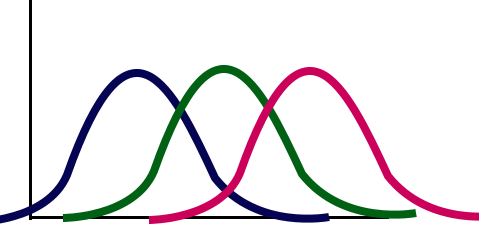
\includegraphics[width=\textwidth]{Cell-B.png}
		\caption{Cell B $\in$ A}
	\end{subfigure}
	~ 
	\begin{subfigure}[b]{0.3\textwidth}
		\centering
		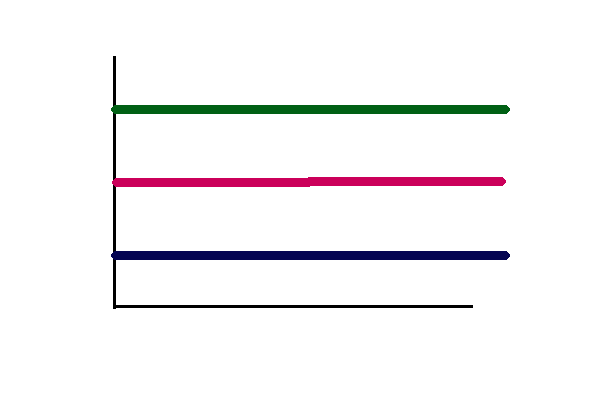
\includegraphics[width=\textwidth]{Cell-C.png}
		\caption{Cell C $\in$ E}
	\end{subfigure}
\end{figure}

\begin{figure}[H]
	\centering
	\begin{subfigure}[b]{0.3\textwidth}
		\centering
		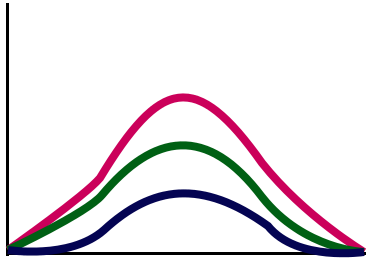
\includegraphics[width=\textwidth]{Cell-D.png}
		\caption{Cell D $\in$ C}
	\end{subfigure}%
	~
	\begin{subfigure}[b]{0.3\textwidth}
		\centering
		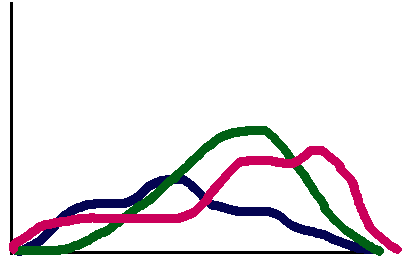
\includegraphics[width=\textwidth]{Cell-E.png}
		\caption{Cell E (Not every neuron shows clear tuning curves)}
	\end{subfigure}
\end{figure}

$R$, $A$ and $E$ have the following relations:
\begin{itemize}
\item $R = A - E$
\item $A = E + R$
\item $E = A - R$
\end{itemize}

How does this information is stored? Say $R$, $A$ and $E$ are encoded by population codes, i.e., by population of units, each tuned to a particular value of that variable. Considering these three variables, the result is seen in Figure~\ref{fig:population}.


\end{document}
